

\chapter{物理学的基礎知識}
\section{波の要素}
ある点での振動が他の点へと伝わっていく現象を\emph{波}という.
波を伝える物質を\emph{媒質}といい,振動によって最初に波が起きた点を\emph{波源}という.

図\ref{fig:sin}は最も基本的な波である\emph{正弦波}である.波形の中で最も高い所を\emph{山},最も低い所を\emph{谷}という.隣り合う山同士,谷同士の間の距離を波長$\lambda$[m]といい,波源から山の高さ,もしくは谷の深さを波の\emph{振幅}という.


\begin{figure}[htbp]
 \begin{center}
  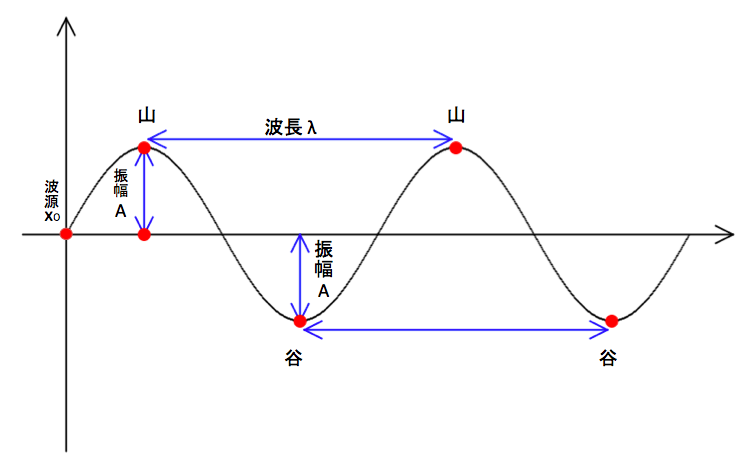
\includegraphics[width=150mm]{../background/lambdasin.png}
 \end{center}
 \caption{波の振幅,波長を示した図.}
 \label{fig:sin}
\end{figure}

\newpage

\section{波の速度と振動数と周期の関係}
1波長分の波が1秒間に発生する回数を\emph{振動数$f$}[1/sec]という.
波の速さ$v$[m]は式(\ref{eq:v})と表すことができる.
\begin{eqnarray}
\label{eq:v}
v=f \lambda
\end{eqnarray}

図\ref{fig:vft}は波の速さ$v$と振動数$f$の関係を示した図である.
\begin{figure}[htbp]
\begin{minipage}[b]{1.0\linewidth}
\centering
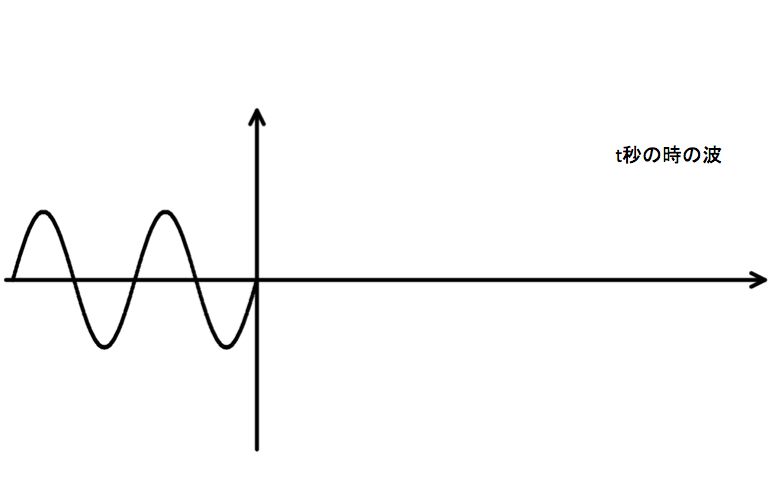
\includegraphics[keepaspectratio, scale=0.42]
  {../background/tminute2.png}
 \subcaption{t秒の時の波.}\label{tminute}
 \end{minipage}
 
\begin{minipage}[b]{1.0\linewidth}
\centering
  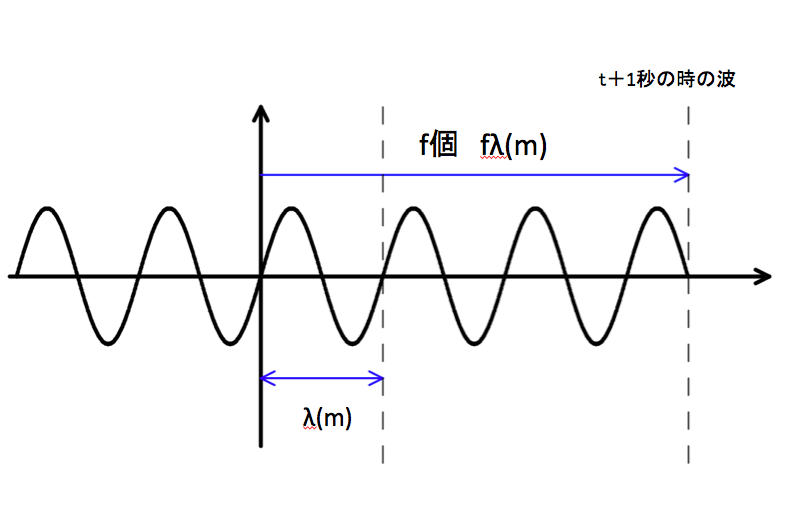
\includegraphics[keepaspectratio, scale=0.42]
  {../background/t+1minute2.png}
 \subcaption{t+1秒の時の波.}\label{t+1minute}
 \end{minipage}
  
  \caption{波の速さ$v$,振動数$f$の関係を示した図.}
 \label{fig:vft}
\end{figure}

また1波長分の波が発生するまでに要する時間を\emph{周期$T$}という.
周期$T$と振動数$f$には式(\ref{eq:t})の関係が成り立つ.
\begin{eqnarray}
\label{eq:t}
T = \frac{1}{f}
\end{eqnarray}

波に対し空気抵抗や摩擦力などの他の外力を一切適用しなければ,周期ごとの波形は完全に一致する.
今回作成するプログラムは教材として用いることや,処理の複雑さに伴う描画速度の低下を考慮し,他の外力を一切適用しないとして波を描写するため,これ以降の記述は全て他の外力が一切適用されていない状態での波を考えているものとする.


\section{正弦波の変位の計算方法}
\label{sec:calculatey}
任意の地点かつ時間における正弦波の変位を計算する際には,以下に挙げる要素が必要である.
\begin{enumerate}
 \item 波長
 \item 波源からの距離
 \item 現在の時間と波源が生成された時間との差
 \end{enumerate}
全ての要素を同時に考慮することは難しいので,1-2の要素と3の要素を分けた上で正弦波の変位を計算する方法を説明する.
計算方法の手順を以下に示す.
\begin{enumerate}
\item 正弦波の任意の地点における位相変化が波源(角度は$0^{\circ}$)の位相変化よりどれだけずれているかを,波源から任意の地点までの距離と波長から算出する.
 \item 目標とする時刻と,波源の位相が$0^{\circ}$に生成された波の位相のずれを算出する.
\item 手順2で求めた位相のずれから手順1で求めた位相のずれを引いたものを$y$とし,$\sin(y)$の値に振幅を掛け合わせる.
 \end{enumerate}

手順1の詳細を以下に示す.
波源の位相が$0^{\circ}$である時の正弦波で考える.
任意の地点をAとする.図\ref{fig:dislam}は波源から地点Aまでの距離を表したものである.波源から目標地点(地点A)までの距離をd1とする.
この時,波は1波長ごとに同じ形をしていることから,地点Aの位相($0^{\circ}$$\sim$$360^{\circ}$)はd1を$\lambda$で割った値に360を掛けることで求めることができる.




\begin{figure}[htbp]
 \begin{center}
  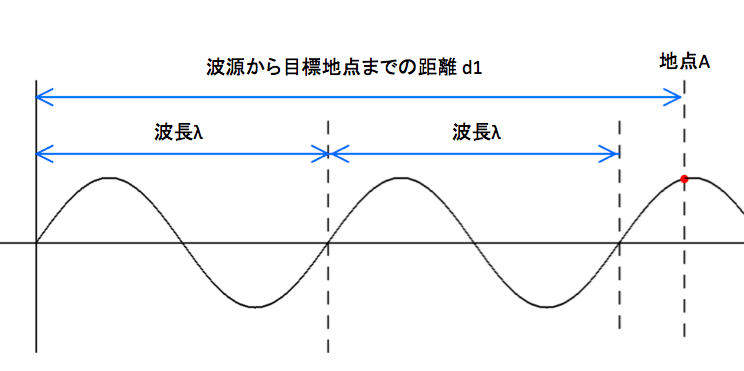
\includegraphics[width=120mm]{../background/dislam1.png}
 \end{center}
 \caption{正弦波における波源と地点Aの関係.}
 \label{fig:dislam}
\end{figure}

図\ref{fig:tezyun1}はある時刻$t$0と,正弦波が$\frac{\lambda}{4}$分だけ進んだ時刻$t$1の正弦波の状態を表したものである.
時刻$t$0の時,波源の正弦波の変位は$\sin(90^{\circ})$である.これに対し,時刻$t$1では目標地点Aの変位が$\sin(0^{\circ})$となり,波源の変位は$\sin(90^{\circ})$となる.つまり目標地点Aの位相変化は波源よりも$90^{\circ}$遅れていることが分かる.よって手順3では波源と目標地点の位相のずれを減算しなければならない.

\begin{figure}[htbp]
 \begin{center}
  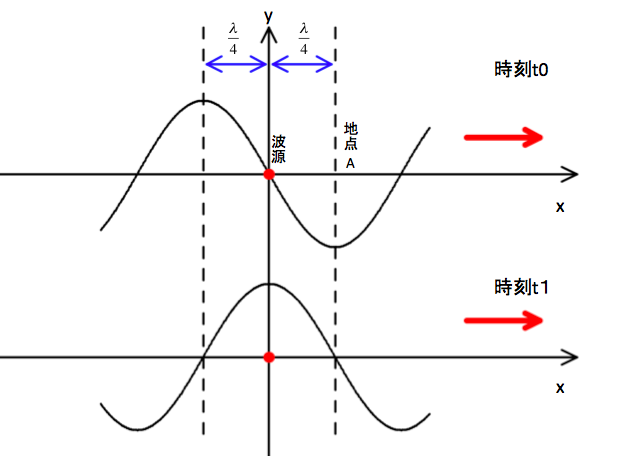
\includegraphics[width=100mm]{../background/tezyun1.png}
 \end{center}
 \caption{波源の位相変化と地点Aの位相変化の関係.}
 \label{fig:tezyun1}
\end{figure}

\newpage


手順2の詳細を以下に示す.
まず
正弦波の波源の位相が$0^{\circ}$である時刻$t0$から$\frac{1}{4}$周期分経過した後の時刻$t1$に波源が生成された例を考える.
図\ref{fig:timeadjust}の上側の青色の波は時刻$t0$の正弦波w0であり,下側の青色の波は時刻$t1$の時の正弦波w1である.また下側の薄い赤色の波は$t0$の正弦波w0である.
w1の波はw0で考えるためには角度のずれを足さなければならない.
w0の任意の点の位相はw1で対応する点の位相よりも$\frac{1}{4}$周期,つまり$90^{\circ}$だけ先に進んでいることが分かる.つまりw1をw0に対応させるために手順3で値を$90^{\circ}$分足さなければならない.



\begin{figure}[htbp]
 \begin{center}
  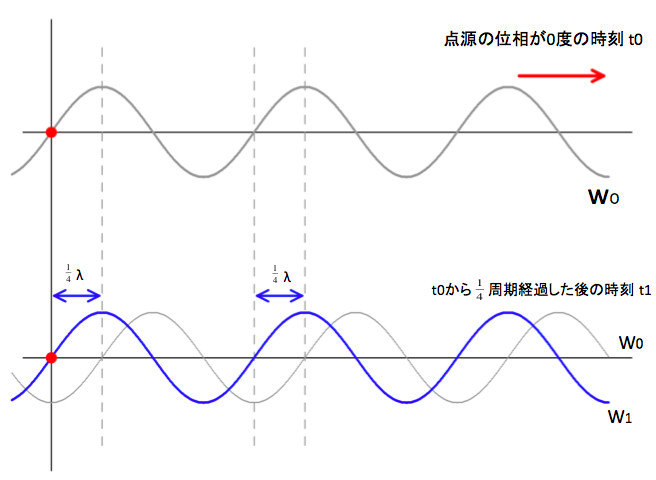
\includegraphics[width=150mm]{../background/timeadjust.png}
 \end{center}
 \caption{経過時間による変位の変化を表した図.}
 \label{fig:timeadjust}
\end{figure}






\newpage
\section{波の独立性と重ね合わせの原理}
図\ref{fig:synwave}(a)は別の波源から生じた2つの波が互いに近づいている様子である.

図\ref{fig:synwave}(b)は2つの波が重なっている様子である.水色の波の変位は,2つの波の変位を足し合わせたものである.このように複数の波が重なり合ってできた波を\emph{合成波}という.
合成波の変位が,重なっているそれぞれの波の変位を足し合わせたものになることを,\emph{重ね合わせの原理}という. また,複数の波が重なり合って弱めあったり強めあったりする現象を波の\emph{干渉}という.

図\ref{fig:synwave}(c)は2つの波が重なった後,離れていく様子である.2つの波は一度重なったにもかかわらず,図\ref{fig:synwave}(a)の時と同じ波形を保っている.このような性質を\emph{波の独立性}という.

\begin{figure}[htbp]
\begin{minipage}[b]{1.0\linewidth}
\centering
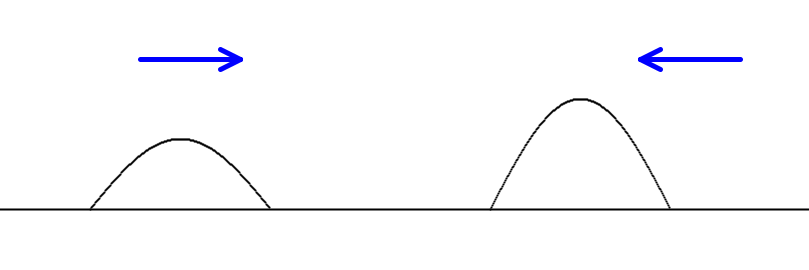
\includegraphics[keepaspectratio, scale=0.45]
  {../background/synwave1.png}
 \subcaption{2つの波が重なる前.}\label{synwave1}
 \end{minipage}
 
\begin{minipage}[b]{1.0\linewidth}
\centering
  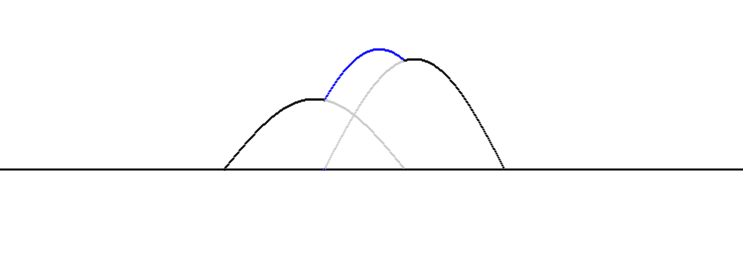
\includegraphics[keepaspectratio, scale=0.45]
  {../background/synwave2.png}
 \subcaption{2つの波が重なっている時.}\label{synwave2}
 \end{minipage}
  
  \begin{minipage}[b]{1.0\linewidth}
\centering
  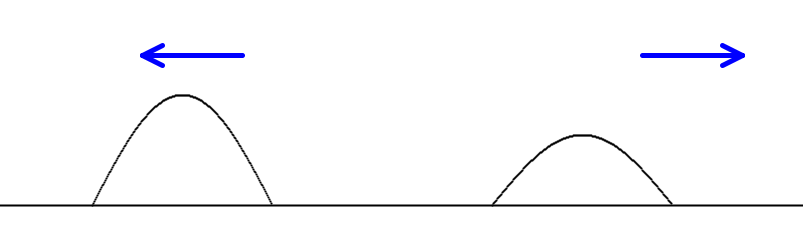
\includegraphics[keepaspectratio, scale=0.45]
  {../background/synwave3.png}
 \subcaption{2つの波が重なった後.}\label{synwave3}
 \end{minipage}
  
  \caption{波の独立性と重ねあわせの原理.}
 \label{fig:synwave}
\end{figure}

\section{ホイヘンスの原理}
同じ時刻に同じ状態の点を結んだ線または面を\emph{波面}という.ある波面とその隣の波面との間隔は波長$\lambda$である.
波面が平面であるものを\emph{平面波}といい,球面状のものを\emph{球面波}という.

\emph{ホイヘンスの原理}とは,任意の波面上の全ての点がそれらを波源とする球面波(素元波)を発生させ,素元波の共通に接する面が次の瞬間の波面を形作るとする理論である.

図\ref{fig:hoihens1},図\ref{fig:hoihens2}はホイヘンスの原理により平面波,球面波が新たな波面を形作る様子を示したものである. 赤い線が波面,赤い点が素元波を生成する点,青い線が素元波としている.
%また図には示していないが,素元波を生成する点はどの波面状にも無数に存在する.

\begin{figure}[thbp]
\begin{minipage}{0.5\hsize}
\begin{center}
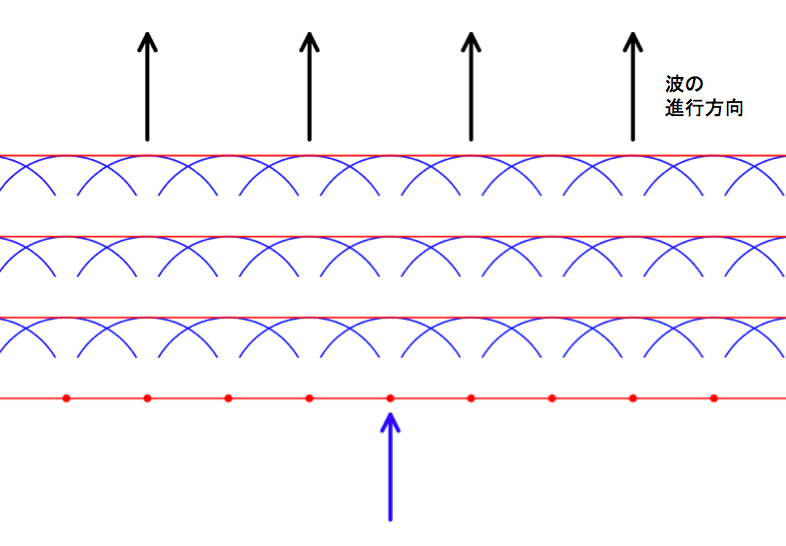
\includegraphics[width=\linewidth]
  {../background/hoihens1.png}
\caption{平面波.}
\label{fig:hoihens1}
\end{center}
\end{minipage}%
\begin{minipage}{0.5\hsize}
\begin{center}
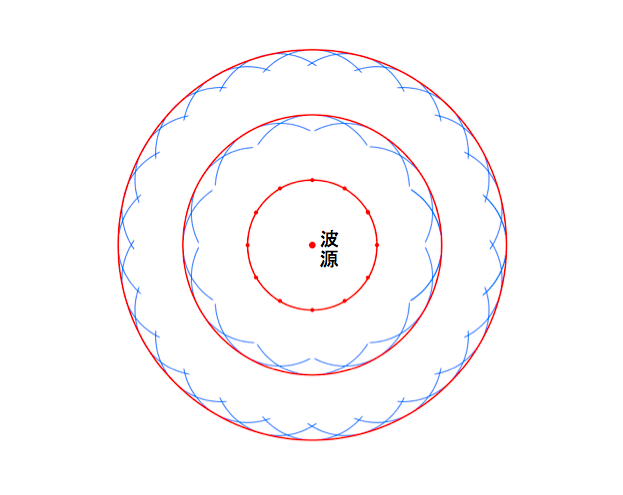
\includegraphics[width=\linewidth]
  {../background/hoihens2.png}
\caption{球面波.}
\label{fig:hoihens2}
\end{center}
\end{minipage}
\end{figure}
\newpage



\section{反射の法則}
まず, 入射波のある端点が点$B_{1}$に到達した時, 点$B_{1}$から素元波が生成される.この時, 素元波は入射波と同じ媒質中を進むため,入射波と同じ速度で進行する. 次に, 入射波の異なる端点が遅れて$A_{2}$点に到達する.その時,$B_{1}B_{2}$点と$A_{1}A_{2}$点の長さは同じであり,三角形ACDと三角形ABDは合同となる. この事から,入射角$i$と反射角$j$が等しくなることがわかる.これを反射の法則という.
\begin{eqnarray}
\label{eq:refraction5}
i=j
\end{eqnarray}


\begin{figure}[htbp]
 \begin{center}
  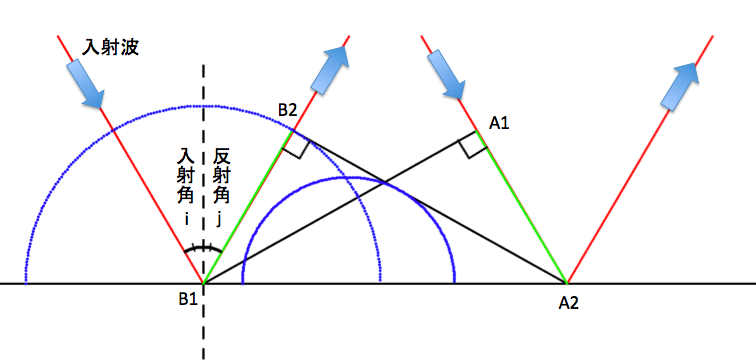
\includegraphics[width=80mm]{../background/reflection1.png}
 \end{center}
 \caption{反射の法則.}
 \label{fig:backreflection}
\end{figure}

\section{屈折の法則}
波の速度は,媒質の種類によって変化する.波がある媒質から別の媒質に進んでいくことで波の速度が変化し,媒質の境界面を境として波の進む方向が変わることを\textgt{波の屈折}という.

\begin{figure}[H]
 \begin{center}
  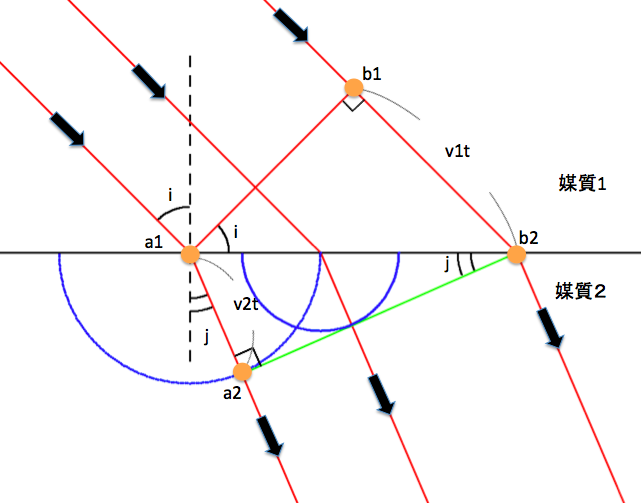
\includegraphics[width=120mm]{../background/backrefraction.png}
 \end{center}
 \caption{ホイヘンスの原理による屈折の説明.}
 \label{fig:backrefraction}
\end{figure}

図\ref{fig:backrefraction}はホイヘンスの原理の考え方を用いて波が屈折する仕組みを示したものである.
%入射波の進行方向と境界面の垂線がなす角を\emph{入射角}(図中の角度$i$),
%屈折波の進行方向と境界面の垂線がなす角を\emph{屈折角}(図中の角度$j$)という.

媒質1,2における波の速さをそれぞれ$v_{1}$, $v_{2}$とし,波面$a_{1}b_{1}$上の点$b_{1}$が$b_{2}$に達するまでの時間を$t$とすると,
\begin{eqnarray}
\label{eq:refraction1}
b_1 b_2=v_1 t
\end{eqnarray}
が成り立つ.この時,時間$t$に$a_{1}$から出た素元波は$v_{2}$の速度で広がるため,
\begin{eqnarray}
\label{eq:refraction2}
a_1a_2=v_2t
\end{eqnarray}
となる.

式(\ref{eq:refraction1}),式(\ref{eq:refraction2})から
\begin{eqnarray}
v_1t=a_1b_2\sin(i) \\ \nonumber
v_2t=a_1b_2\sin(j)
\label{eq:refraction3}
\end{eqnarray}
が導出される.
式(2.6)と屈折によって波の振動数は変化しないことから
式(\ref{eq:refraction4})が成り立つ.
\begin{eqnarray}
\label{eq:refraction4}
\frac{\sin(i)}{\sin(j)}=\frac{v1}{v2}=\frac{\lambda1}{\lambda2}
\end{eqnarray}

式(\ref{eq:refraction4})の$\frac{v1}{v2}$や$\frac{\lambda1}{\lambda2}$は媒質1,2の物質によって決まる一定の値である.これを\emph{屈折率$n$}と定義すると式(\ref{eq:refraction5})が成り立つ.これを\emph{屈折の法則}という.

\begin{eqnarray}
\label{eq:refraction5}
\frac{v1}{v2} = n_{12}
\end{eqnarray}



\section{回折現象}
\subsection{ホイヘンスの原理による回折現象の説明}
波が障害物の裏まで回り込む性質を波の\emph{回折}という.
図\ref{fig:difraction}(a)は障害物間の間隔が広い時の波の様子を示している.この時,隙間の中央部分は平面波,両端部分は円形波として伝わる.
一方,図\ref{fig:difraction}(b)のように障害物間の間隔が狭い時は,平面波の領域が小さくなり,波の形は円形波に近くなる.
\begin{figure}[H]
\begin{minipage}[b]{1.0\linewidth}
\centering
  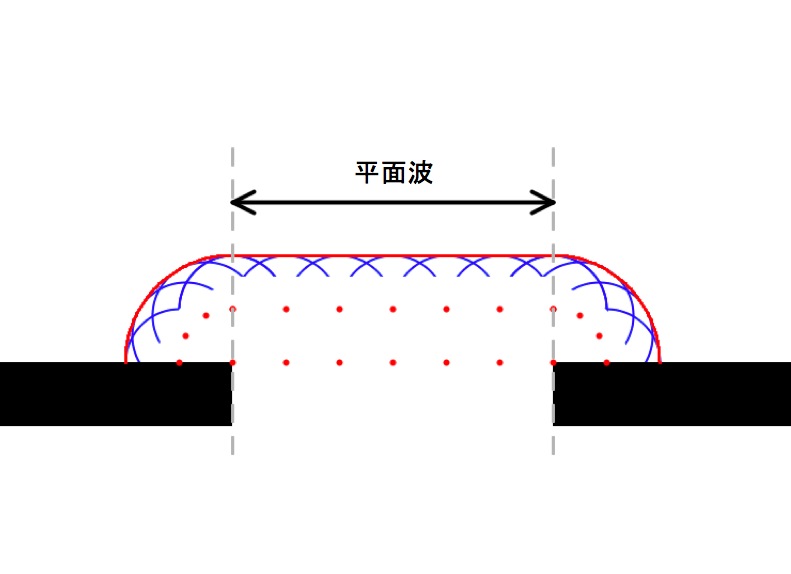
\includegraphics[keepaspectratio, scale=0.45]
  {../background/difraction2.png}
 \subcaption{間隔が広い時.}\label{difraction1}
 \end{minipage}
  
  \begin{minipage}[b]{1.0\linewidth}
\centering
  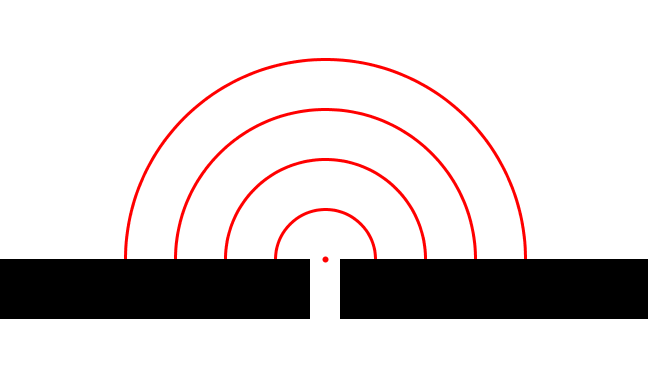
\includegraphics[keepaspectratio, scale=0.45]
  {../background/difraction1.png}
 \subcaption{間隔が狭い時.}\label{difraction2}
 \end{minipage}
  
  \caption{隙間の間隔の広さによる波の形の差異.}
 \label{fig:difraction}
\end{figure}








\subsection{実際の回折現象}
図\ref{fig:difraction}(a),(b)では波同士の干渉や波の波長を考慮していない.実際は図\ref{fig:difraction}(a)のような状況だと,隙間の両端部分は各波の位相のずれで打ち消しあってしまうため,回折現象はほとんど見られない. 隙間の間隔が小さく,波長の長さが長い方が回折現象は起こりやすい.実際の回折現象をシミュレーションした結果は\ref{defraction}節に記す.





